%!TEX root = ../thesis_a4.tex

\chapter{Background}
\label{sec:SOA}

\section{Introduction}
\label{sec:SOA:Introduction}

The literature review presented in this chapter is divided in three parts. Each part is focused on each one of main fields of research where this thesis is framed: Natural Language Processing (NLP), Recommender Systems (RS), and Music Information Retrieval (MIR).
First, we summarise existing work on several areas of Natural Language Processing, with special focus on its application to the music domain. 
We define what a knowledge base (KB) is and the different existing types. Moreover, we deepen into the available knowledge bases that contain music information.
Then, we explain what entity linking is and briefly describe some state-of-the-art systems. Additionally, we outline different existing approaches for relation extraction. 
Hereafter, we briefly explain the different main approaches used in Recommender Systems. Then, we enumerate the main available works related to semantic-based approaches for recommendation.
Finally, we dig into the available literature on Music Information Retrieval. More specifically, we first review the state-of-the-art in text-based and semantic-based approaches. Then, we focus on three specific tasks: music genre classification, artist similarity, and music recommendation.
%. First, we recapitulate existing work about music genre classification, with a special focus on text-based approaches.
%Second, we illustrate existing text-based apporaches for artist similarity.
%Finally, we outline the different apporaches that have been proposed about semantic-based recommender systems and cold-start music recommendation.


\section{Natural Language Processing}
\label{sec:SOA:nlu}

Natural Language Processing (NLP) is a field of study that focuses on the interactions between human language and computers. One of the main subtopics of NLP is Natural Language Understanding (NLU), which deals with machine reading comprehension.
Knowledge Representation and Reasoning is a key enabler of Intelligent Systems \citep{Suchaneketal2007}, and plays an important role in NLU \citep{BaralandDeGiacomo2015}.
In this dissertation, we focus on an important aspect of NLU, which is \textit{how to make sense} of the data that is generated and published online on a daily basis. This data is mostly produced in human-readable format, which makes it unsuitable for automatic processing. Considering that deep understanding of natural language by machines seems to be very far off \citep{CambriaandWhite2014}, there is great interest in formalizing unstructured data, and knowledge bases are a paradigmatic example of large-scale content processed to make it machine readable.

Information extraction is the task of automatically extracting structured information from unstructured or semi-structured text sources. It is a widely studied topic within the NLP research community \citep{cowie1996information}.
A major step towards understanding language is the extraction of meaningful terms (entities) from text as well as relationships between those entities. This statement involves two different tasks. First, to determine the identity and category of entity mentions present in text. This task is called named entity recognition. However, when this task involves a latter step of disambiguation of entities against a knowledge base it is called named entity disambiguation or entity linking. Second, to identify and annotate relevant semantic relations between entities in text, which is called relation extraction.

The work described in this thesis strongly focuses on the exploitation of linguistic and semantic properties of text collections. For this reason, we deem relevant to cover related work in the following areas: (1) knowledge base construction and curation; (2) music knowledge bases; (3) entity linking, and (4) relation extraction.


\subsection{Knowledge base construction}
\label{sec:SOA:nlu:kbs}

We may define a knowledge base as a repository of knowledge organized in a predefined taxonomic or ontologic structure, potentially compatible with other knowledge bases, thus contributing to the Linked Open Data initiative\footnote{\url{http://linkeddata.org/}}. These knowledge bases may be designed to represent unconstrained knowledge, or a single domain of interest. This representation is formalized either manually, automatically, or with a combination of both.

We understand language by making sense of the connections between words, concepts, phrases and thoughts \citep{Havasietal2007}. Knowledge bases constitute a resource for encapsulating this knowledge. Previous efforts on knowledge base construction may be characterized as: (1) handcrafted knowledge bases; (2) integrative projects (automatic in design, but reliant on manually validated data); and (3) fully automatic, also in the relation extraction process.

Among the first group, the best known is probably \texttt{WordNet} \citep{Miller1995}, a lexical database which groups concepts in ``synonym sets'', and encodes predefined relations among them such as \textit{hyponymy/hypernymy}, \textit{meronymy}, \textit{holonymy}, or \textit{instantiation}. Manually constructed knowledge bases, however, are mostly developed in specific domains, where the degree of ambiguity is lower and there is more availability of trained knowledge engineers.

Next, integrative projects are probably the most productive, as they are the most ambitious attempts in terms of content coverage and community involvement, not only users, but also contributors. Examples of these include \texttt{Yago} \citep{Suchaneketal2007}, an automatically created knowledge base derived from integrating \texttt{Wikipedia} and \texttt{WordNet}; \texttt{DBpedia} \citep{Lehmanetal2014}, a collaboratively maintained project aimed at exploiting information present in \texttt{Wikipedia}, both structured and in free text; \texttt{Freebase} \citep{Bollacketal2008}, also a collaborative effort mainly based on extracting structured knowledge from \texttt{Wikipedia}; or \texttt{BabelNet} \citep{NavigliPonzetto2012}, a semantic network which started as a seamless integration of \texttt{Wikipedia} and \texttt{WordNet}, and today constitutes the largest multilingual repository of words and senses.

With regard to the third group we refer to approaches where knowledge is obtained automatically. 
%Usually, these are framed within the \textit{Open Information Extraction} (OIE) paradigm \citep{Bankoetal2007}, which can be (roughly) summarized as (1) reading the web, (2) learning facts, (3) scoring them; and (4) structuring them according to predefined semantic criteria. 
Endeavours in this area include \texttt{TextRunner} \citep{Bankoetal2007}, widely regarded as the first \textit{Open Information Extraction} (OIE) system; \texttt{ReVerb} \citep{Fader2011}, particularly designed to reduce noise while keeping a wide coverage, thanks in part to a set of syntactic and lexical constraints; \texttt{NELL} \citep{Carlson2010}, which incorporates semantic knowledge in the form of a handcrafted taxonomy of entities and relations; \texttt{PATTY} \citep{Nakasholeetal2012} and \texttt{WiseNet} \citep{MoroandNavigli2012,MoroandNavigli2013}, in which a shared vision to integrate semantics is applied both at the entity and relation level; \texttt{DefIE} \citep{DelliBovietal2015b}, a recent development in OIE tested on the whole set of \texttt{BabelNet} glosses; and \texttt{KB-Unify} \citep{DelliBovietal2015}, not an actual information extraction implementation, but rather a unification framework for knowledge bases.

%Another key aspect of automatic knowledge base generation, in addition to semantics, is \textit{how relations between entities are captured}. From rule-based linguistically motivated approaches to machine learning methods, the general trend seems to extract as many facts as possible, with as much accuracy as possible, and keeping the degree of supervision low.

%Previous work exploited combinations of surface and part-of-speech patterns \citep{Bankoetal2007} or regular expressions \citep{Fader2011}, as well as rules based on shallow parsing \citep{MoroandNavigli2012}. Furthermore, there are a number of contributions exploiting syntactic information in the form of syntactic dependencies, a linguistic formalism \citep{Tesniere1959} that represents sentences as trees where each relation is bi-lexical and non phrasal, and where in general, syntactically important words (subject, verb, or direct object) appear higher in the tree. Syntactic dependencies have been extensively used in \texttt{RE}, e.g. in supervised machine learning settings for computational lexicography \citep{EspinosaandSaggion2014}. They have played a role also in Entity Linking (EL), e.g. enabling syntactic tree traversal between entities \citep{BunescuandMooney2005}, providing smallest spanning subtrees subsuming two entities \citep{CulottaSorensen2004}, or as part of a rule-based OIE system \citep{Gamallo2012}.

\subsection{Music knowledge bases}\label{sec:SOA:nlu:mkbs}

\texttt{MusicBrainz} and \texttt{Discogs} are two paramount examples of manually curated music knowledge bases. They are not strictly knowledge bases, but open music encyclopedias of music metadata, which are built collaboratively and are openly available. \texttt{MusicBrainz}, in addition, has been published as Linked Data by the \texttt{LinkedBrainz} project\footnote{\url{http://linkedbrainz.org/}}.

As for generic knowledge bases based on \texttt{Wikipedia}, such as the ones described earlier, these include a remarkable amount of music data, such as artist, album, and song biographies; definitions of musical concepts and genres; and articles about music institutions and venues. However, their coverage is biased towards the best known artists, and towards products from Western culture. Finally, let us refer to the notable case of \texttt{Grove Music Online}\footnote{\url{http://www.oxfordmusiconline.com}}, a music encyclopedia containing over 60k articles written by music scholars. However, it has the drawback of not being freely open, as it runs by subscription.
Other than the aforementioned curated repositories, to the best of our knowledge, there is not a single automatically learned open music knowledge base. A first step in this direction is taken in this disertation.
%was taken in \citep{Sordo2015,Oramas2014}, applying \textsc{RE} techniques to big datasets of music related texts extracted from the web. Moreover, in \citep{Oramas2015b}, a Flamenco music knowledge bases is created by combining data from curated knowledge bases and information extracted from blogs and websites.

Despite their scarcity, knowledge bases with music information are becoming increasingly popular in MIR applications, such as artist similarity and music recommendation \citep{Celma2008,Leal2012,Ostuni2013}.
Music knowledge bases have also been exploited as sources of explanations in music recommender systems. %According to~\citep{CelmaandHerrera2008}, giving explanations of the recommendations provides transparency to the recommendation process and increases the confidence of the user in the system. 
For instance, in \citep{Passant2010}, explanations of recommendations are created by exploiting \texttt{DBpedia}'s graph.%, whilst in \citep{Sordo2015}, explanations are based on an automatically learned music knowledge bases. 


\subsection{Entity linking}
\label{sec:SOA:nlu:entity_linking}

The advent of large knowledge repositories and collaborative resources has contributed to the emergence of entity linking (EL), i.e. the task of discoveing mentions of entities in text and link them to a suitable knowledge repository \citep{Moroetal2014}. 
It encompasses similar subtasks such as named entity disambiguation \citep{BunescuandPasca2006}, which is precisely linking mentions of entities to a knowledge base, or wikification \citep{MihalceaandCsomai2007}, specifically using Wikipedia as knowledge base.
Another highly related technique is word sense disambiguation \citep{stevenson2003word}. It's main task is to identify which sense of a word (i.e. meaning) is used in a sentence, when the word has multiple meanings.

There have been a great development of entity linking systems for unconstrained domains. Among these systems we focus on three of them in this thesis:

\noindent \textbf{DBpedia Spotlight} \citep{Mendes2011} is a system for automatically annotating text documents with DBpedia URIs, finding and disambiguating natural language mentions of DBpedia resources. DBpedia Spotlight is shared as open source and deployed as a Web service freely available for public use\footnote{https://github.com/dbpedia-spotlight/dbpedia-spotlight/}.
%DBpedia Spotlight gives as a result the DBpedia uri, start and end char positions, the value of the rdf:type property, and a confidence score.\\

%\vspace{-0.2cm}
\noindent \textbf{TagMe} \citep{Ferragina2012} is an entity linking system that matches terms with Wikipedia link texts and disambiguates them using the Wikipedia in-link graph. Then, it performs a pruning process by looking at the entity context. TagMe is available as a web service~\footnote{https://tagme.d4science.org/tagme/}.
%Tagme output provides the start and end char position, the Wikipedia page id, the Wikipedia categories and a confidence score. \\

%\vspace{-0.2cm}
\noindent \textbf{Babelfy} \citep{Moroetal2014b} is an entity linking and word sense disambiguation system based on non-strict identification of candidate meanings (i.e. not necessarily exact string matching), together with a graph based algorithm that traverses the BabelNet graph and selects the most appropriate semantic interpretation for each candidate~\footnote{http://babelfy.org/}.
%Babelfy output provides the BabelNet synset and the word index. If the synset references to a Wikipedia page, it returns the Wikipedia url, the DBpedia uri and the Wikipedia categories. If it points to WordNet, it yields the nçame of the equivalent WordNet synset.

In the context of Open Data, the need for benchmarking datasets and evaluation frameworks for entity linking is clear. However, while general purpose datasets and benchmarks exist \citep{Usbeck2015}, dealing with highly specific domains (e.g. chemistry) or ever-evolving areas (e.g. video games or music) poses a greater challenge due to linguistic idiosyncrasies or under-representation in general purpose knowledge bases. This is true in the music domain as well, where available data is scarce \citep{Gruhl2009}.
Among the few works on entity linking for the music domain, let us refer to \cite{Gruhl2009}, who describe an approach for detecting musical entities from MusicBrainz in informal text. In addition, \cite{Zhang2009} describe a system for musical entity linking in the Chinese language based on Hidden Markov Models. %Finally, \citep{Oramas2015} describe an entity linking system for recognizing musical entities in a relation extraction pipeline.

There is a number of evaluation benchmarks for general purpose entity linking systems. \citep{Cornolti2013} put forward a benchmarking framework for comparing entity linking systems, leveraging Wikipedia, and a hierarchy of entity linking problems together with a set of novel measures. \citep{Rizzo2014} and \citep{Gangemi2013} provide evaluation reports on the performance of different state-of-the-art named entity recognition and entity linking systems. Finally \citep{Usbeck2015} present GERBIL, an evaluation framework for entity linking based on \citep{Cornolti2013}.
%It is an open-source and extensible framework that allows evaluating tools against different datasets.


\subsection{Relation extraction}
\label{sec:SOA:nlu:relation_extraction}

%TODO-LUIS: go through this section one more time [a little bit about relation extraction (plus maybe NER, dependency parsing) (check the review paper by Nguyen Bach and Sameer Badaskar, ``A Review of Relation Extraction'' \citep{Bach2007})]

%Vast amount of unstructured text on the web. One way to ... is to structure the text by annotating in such a way that it can be use/manipulated by algorithms/machines?

A large portion of the knowledge contained in the web is stored in unstructured natural language text. In order to acquire and formalize this heterogeneous knowledge, methods that automatically process this information are in demand. Extracting semantic relations between entities is an important step towards this formalization \citep{Wang2008}. Relation Extraction (RE) is an established task in Natural Language Processing~\citep{Bach2007}. It has been defined as the process of identifying and annotating relevant semantic relations between entities in text \citep{JiangZhai2007}. 

Relation Extraction approaches are often classified according to the level of supervision involved.
%Relation Extraction systems are often classified into Traditional and Open Relation Extraction.
%In traditional Relation Extraction (RE), the vocabulary of extracted relations is defined a priori, i.e. in a domain ontology or an extraction template.
Supervised learning is a core-component of a vast number of relation extraction systems, as they offer high precision and recall. However, the need of hand labeled training sets makes these methods not scalable to the thousands of relations found on the Web \citep{Hoffmann2011}.
%semi-supervised and bootstrapping approaches have gained popularity \citep{Bach2007}.
More promising approaches, called semi-supervised approaches, bootstrapping approaches, or distant supervision approaches do not need big hand labeled corpus, and
%do not need a complete hand labeled training corpus. These approaches
often rely on existent knowledge bases to heuristically label a text corpus (e.g.,~\citep{Carlson2010,Hoffmann2011})
%, and use it to learn a probabilistic model ( (such as~\citep{Hoffmann2011}) ) . A similar approach is used by the NELL system \citep{Carlson2010}, but instead of learning a probabilistic model, it is based on a bootstrapping approach.
%Multi-instance learning approaches are combined with distant supervision to combat the problem of ambiguously-labeled training data for the identification of overlapping relations \citep{Hoffmann2011, Xu2013}.
%This is because supervised training of accurate relation extractors is costly, requiring a high number of annotated examples.
%, or it is learned from hand tagged training examples.
%In contrast with traditional Relation Extraction,

%Unsupervised approaches do not need any annotated corpus. In \citep{Eichler2008} verb relations involving a subject and an object are extracted, using simplified dependency trees in sentences with at least two named entities. These approaches can process very large amounts of data, however, the resulting relations are hard to map to ontologies \citep{Augenstein2014}.
Open information extraction (OIE) methods do not require an annotated corpus nor a pre-specified vocabulary, as they aim to discover all possible relations in the text \citep{Banko2007}.
However, these unsupervised methods have to deal with uninformative and incoherent extractions. In \citep{Fader2011} part-of-speech based regular expressions are introduced to reduce the number of these incoherent extractions. Less restrictive pattern templates based on dependency paths are learned in \citep{Mausam2012} to increase the number of possible extracted relations.
%Extracting semantic relations between entities is an important step towards this formalization \citep{Wang2008}. Relation Extraction is an established task in Natural Language Processing~\citep{Bach2007}. It has been defined as the process of identifying and annotating relevant semantic relations between entities in text \citep{JiangZhai2007}. It typically consists of two steps. First, entities are identified in the text. The identification can be achieved by using a well known NLP technique called Named Entity Recognition. Named Entity Recognition (NER) is the process of identifying proper nouns in running text, such as persons, locations or organizations \citep{Bach2007}. This problem has been studied extensively and the most commonly proposed solutions use linguistic grammar based techniques or machine learning approaches~\citep{Nadeau2007}. The latter step in Relation Extraction involves the indentification of a semantic relation between two named entities. Supervised approaches either rely heavily on features obtained from careful linguistic analysis, like Part-of-Speech tagging or syntactic parsing, or exploit a structured representation of natural language (e.g. sequences or trees) \citep{JiangZhai2007}. Although supervised learning is a core-component of a vast number of RE systems, semi-supervised and bootstrapping approaches have gained popularity \citep{Bach2007}. This is because supervised training of accurate relation extractors is costly, requiring a high number of annotated examples.
%Semi-supervised methods, on the other hand, only need a small number of labeled examples, which in some cases can cause a drop in accuracy \citep{Carlson2010}.
%In Traditional Relation Extraction, the vocabulary of extracted relations is defined a priori, i.e. in a domain ontology or an extraction template, or it is learned from hand tagged training examples. On the other hand, Open Relation Extraction methods do not require a pre-specified vocabulary, as they aim to discover all possible relations in the text \citep{Banko2007}. However, these methods have to deal with uninformative and incoherent extractions. In ReVerb \citep{Fader2011} part-of-speech based regular expressions are introduced to reduce the number of these incoherent extractions. Less restrictive pattern templates based on dependency paths are learned in OLLIE \citep{Mausam2012} to increase the number of possible extracted relations.

%The aim of this paper is to show that when the analyzed unstructured text sources are domain specific (in this case music) and reviewed by a group of domain experts, unsupervised approaches using simple rules can map extracted relations with an existing knowledge base with a high precision.

% There are some approaches about how to extract those relations, but generally they formulate the task as a binary classification problem.

%The above examples refer to Traditional Relation Extraction, where relations to be extracted should be manually defined a priori from text. On the other hand, Open Relation Extraction methods do not require to manually define the relations to be extracted, however, they use to have lower recall. Both methods can be also combined, extracting relations patterns automatically and using those extracted pattern as input of Traditional Relation Extraction systems \citep{Mohamed2011}.

%One of these structured representations can be obtained from Dependency Parsing, which provides a tree-like syntactic structure of a sentence based on the linguistic theory of
%Another way of obtaining relations between entities in the text is by using a technique called Dependency Parsing.
%In our work we use an NLP technique called Dependency Parsing in the relation extraction process. 
Dependency parsing is an NLP technique that provides a tree-like syntactic structure of a sentence based on the linguistic theory of Dependency Grammar \citep{Tesniere1959}. One of the outstanding features of Dependency Grammar is that it represents binary relations between words \citep{BallesterosNivre2013}.%, where there is a unique edge joining a node and its parent node (see Fig. \ref{fig:sampletree} for the full parsing of an example sentence).
Dependency relations have been successfully incorporated to relation extraction systems. For example, \cite{BunescuandMooney2005} describe and evaluate a relation extraction system based on shortest paths among named entities. \cite{CulottaSorensen2004} focus on the smallest dependency subtree in the sentence that captures the entities involved in a relation, and \cite{Gamallo2012} propose a rule-based dependency-parsing open information extraction system. Moreover, in \cite{Nakasholeetal2012,MoroandNavigli2012,DelliBovietal2015b} syntactyc and semantic information is exploited to reduce inconsistent relations, by means of the combination of dependency parsing and entity linking techniques.


\section{Recommender Systems}
\label{sec:SOA:recommendation}

%Information overload in modern Web applications challenges users in their decision-making tasks. 
%Recommender systems have emerged in the last years as fundamental tools in assisting users to find, in a personalized manner, what is relevant for them in overflowing knowledge spaces. 
The main objective of a recommender system is to predict the \textit{rating} or \textit{preference} that a user would give to an item. By doing so, its mision is to provide suggestions for items to be of use to a user \citep{ricci2011introduction}. \textit{Item} is the general term used to denote what the system recommends to users (e.g. song, album, video, book).

\begin{figure}
	\centering
	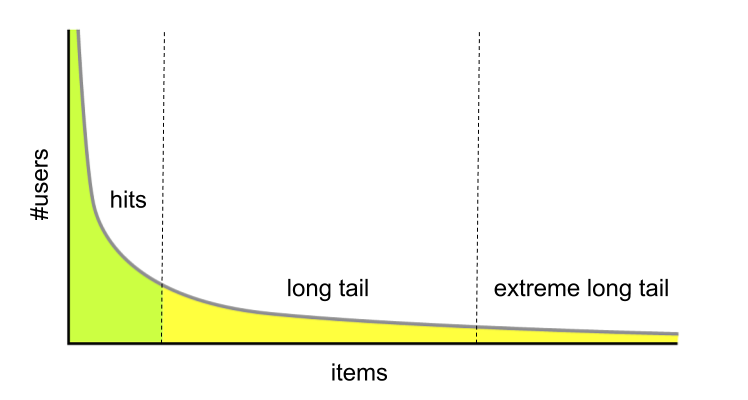
\includegraphics[width=0.6\textwidth]{ch02_soa_pics/Long_tail.png}
	\caption{Long tail distribution.\label{fig:soa:longtail}}
\end{figure}

Within the recommender systems arena, there are two main approaches for computing recommendations: collaborative filtering and contend-based ones.
The most popular is collaborative filtering which provides recommendations to a user by considering the preferences of other users with similar tastes. 
Matrix factorization techniques are currently collaborative filtering state-of-the-art \citep{Koren2009}. 
As collaborative filtering methods rely only on users feedback information, they may suffer from the so-called \textit{cold-start} problem \citep{Saveski2014}. That is, when new items are introduced in the system, they can not be initially recommended as there is no feedback information related to them.
In addition, most popular items tend to attract most of the recommendations in collaborative filtering approaches. The relation between items and popularity is tipically represented as a \textit{long tail} distribution \citep{anderson2006long} (see Figure~\ref{fig:soa:longtail}). A large number of items in the catalog normally receive few interacitons from users, so they are hadrly recommended to users. This items are often called \textit{long tail} items. These less popular items may be promoted by priming other evaluation measures rather than prediction accuracy, such as novelty or diversity.
However, an even larger set of items in large catalogs receive almost none interactions. These \textit{extreme long tail} items are in practice as cold-start items, as the number of interactions is smaller than the minimum value requiered for collaborative filtering methods.

Contrary to collaborative filtering, content-based methods \citep{Mooney1999} rely only on item features, and recommendations are based on similarity between such features. Content-based methods does not suffer from the cold-start problem and are not biesed towards popular items. However, collaborative filtering methods tend to perform better when measuring the overall accuracy of the prediction \citep{pilaszy2009recommending}.
%Content-based systems recommend items sharing similar features to those a user has preferred in past.
Finally, hybrid methods \citep{Burke2002} try to combine the best of both worlds, combining both item-content and item-user feedback. 
%Both approaches can be combined to build hybrid systems \cite{Burke2002}. 
When available, the usage of side information about items has proven to boost the performances of pure collaborative filtering techniques \cite{Ning12}. %Furthermore, many works in the past \cite{mobasher2004,Cantador08amultilayer,Semeraro2009,Anand2007} have raised the problem of introducing semantics in content item representations, usually using ontologies, to mitigate the issues of pure keyword- and attribute-based representations.

%Recommender systems can be broadly classified into collaborative filtering (CF), content-based, and hybrid methods. Collaborative filtering methods \citep{Koren2009} use the item-user feedback matrix and predictions are based on the similarity of user or items profiles. Content-based methods \citep{Mooney1999} rely only on item features, and recommendations are based on similarity between such features. Finally, hybrid methods \citep{Burke2002} try to combine both item content and item-user feedback.


\subsection{Semantic-based approaches}
\label{sec:SOA:mir:recommendation:semantic}

Ontology-based and semantics-aware recommendation systems have been proposed in many works in the past. 
%The usage of ontologies to improve recommendation systems has been proposed in many works in the past. 
In \citep{Middleton_2009} an ontological recommender system is presented that makes use of semantic user profiles to compute collaborative recommendations with the effect of mitigating cold-start and improving overall recommendation accuracy. 
In \citep{mobasher2004} the authors present a \textit{semantically enhanced collaborative filtering} approach, where structured semantic knowledge about items is used in conjunction with user-item ratings to create a combined similarity measure for item comparisons. 
In \citep{Ziegler2004} taxonomic information is used to represents the user's interest in categories of products. Consequently, user similarity is determined by common interests in categories and not by common interests in items. 
In \citep{Anand2007} the authors present an approach that infers user preferences from rating data using an item ontology. The system collaboratively generates recommendations using the ontology and infers preferences during similarity computation. 
Another hybrid ontological recommendation system is proposed in \citep{Cantador08amultilayer} where user preferences and item features are described by semantic concepts to obtain users' clusters corresponding to implicit \textit{Communities of Interest}.
In all of these works, the experiments prove an accuracy improvement over traditional memory-based collaborative approaches especially in presence of sparse datasets. 

In the last few years with the availability of Linked Open Data (LOD) datasets, a new class of recommender systems has emerged which can be named as LOD-based recommender systems. 
One of the first approaches that exploits Linked Open Data for building recommender systems is \citep{HeitmannH10}. 
In \citep{Fernandez-Tobias2011} the authors present a knowledge-based framework leveraging DBpedia for computing cross-domain recommendations. 
In \citep{DMOR12,DMORZ12} a model-based approach and a memory-based one to compute content-based recommendations are presented leveraging LOD datasets. Another LOD content-based method is presented in \citep{ODMD14a} which defines a neighborhood-based graph kernel for matching graph-based item representations. 
Two hybrid approaches have been presented lately. In \citep{Ostuni2013} the authors show how to compute top-N recommendations from implicit feedback using linked data sources and in \citep{Khrouf2013} the authors propose an event recommendation system based on linked data and user diversity. 
%In \citep{Rowe1} the authors propose a semantic-aware extension of the SVD++ model, named SemanticSVD++, which incorporates semantic categories of items into the model. The model is able also to consider the evolution over time of user's preferences. 
Finally, another interesting direction about the usage of LOD for content-based RSs is explored in \citep{MustoSLG14} where the authors present Contextual eVSM, a content-based context-aware recommendation framework that adopts a semantic representation based on distributional semantics and entity linking techniques.% In particular entity linking is used to detect entities in free text and map them to LOD.


\section{Music Information Retrieval}
\label{sec:SOA:mir}

As stated in Section~\ref{sec:intro:nlp}, Music Information Retrieval (MIR) is a multidisciplinary field of research that is concerned with the extraction, analysis, and usage of information about music. %Traditionally, MIR has been more focused on the use of audio content, underestimating other sources of information. However, in recent years several studies have showed the benefits of using other modalities, as well as their combination in multimodal approaches \cite{Schedl2014}. 
Although MIR approaches have been traditionally focused on audio content, there have been a growing interest in text-based and multimodal approaches along the last decade. However, most of these text-based approaches are focused on low and mid-level text representations, ignoring the full epistemic potential expressed in texts. In addition, most of audio-based approaches have traditionally relied on handcrafted features, underexploring factors of variability behind the data.
In this dissertation we focus on knowledge-based and representation learning approaches applied to three MIR tasks: music genre classification, artist similarity, and music recommendation.

\subsection{Text-based approaches}

Early work on NLP in the context of MIR is related to the extraction of music artist information from artist-related web pages, using search engines to gather those pages and then parsing their DOM trees \citep{Cohen2000}. Other studies \citep{Ellis2002,Whitman2002} use weighted term profiles based on specific term sets for recommendation and classification tasks. 
%Early work also on multimodal approaches \cite{} combines 
Co-occurrence of artist names in web pages content and page count based on results provided by search engines have been used for artist similarity and recommendation tasks \citep{Schedl2005}. Song lyrics \citep{laurier2008multimodal,corona2015exploration} and tweets \citep{hauger2013million,schedl2012mining} are other commonly used text sources in MIR. %The number of publications related to this topic have been increasing along the years \cite{}. 
More detailed information about text-based approaches applied to MIR problems can be found in \cite{Knees2013, Schedl2014}.

There have been also some initial atempts to work with mid and high-level text representations in the context of MIR. In \cite{Sordo2012}, a methodology for extracting semantic information from music-related forums is proposed, inferring semantic relations from the co-occurrence of musical concepts in forum posts. 
%In \cite{Sordo2013}, a set of semantic facets is automatically obtained and anchored upon the structure of Wikipedia, and tags from the folkosonomy of \texttt{Last.fm} are then categorized with respect to the obtained facets. 
In \cite{Knees2011} a methodology to automatically extract semantic information and relations about musical entities from arbitrary textual sources is proposed. In \cite{TataandDiEugenio2010} a method to extract information about indidual songs from album reviews is proposed, combining syntactic, semantic and sentiment analysis. Finally, the C@amerata task \cite{sutcliffe2016c, sutcliffe2015}, part of the MeidaEval evaluation campaigns from 2013 to 2017, is focused on music Question \& Answering (Q\&A) systems. In this task the input is a natural language phrase, together with a music score in MusicXML, and the required output should be one or more matching passages in the score.

There have been also some interesting works trying to understand the semantics behind the audio signal using natural language text. In this sense, \cite{Whitman2004} combines text analysis with acoustic descriptors in order to automatically generate music reviews from the audio signal. In \cite{koduri2014culture}, culturally relevant and musically meaningful information about melodic intervals extracted from audio and text are structured in a formal knowledge representation and exploited to compute simiarity measures for the discovery of musical entities.
%\cite{Kolozali2013} shows a method for the automatic creation of an ontology of musical instruments using formal concept analysis over audio features. 

\subsection{Semantic-based approaches}
\label{sec:SOA:mir:semantics}

Semantic representations have been also studied in the context of MIR, but instead of extracted from text, they are typically retrieved from online knowledge repositories. For instance, in \cite{Sordo2013} a set of semantic facets is automatically obtained and anchored upon the structure of Wikipedia, and tags from the folkosonomy of \texttt{Last.fm} are then categorized with respect to the obtained facets. In \cite{Celma:ISWC06}, information from different sources is gathered in a central knowledge repository following the Semantic Web principles and using Friend of a Friend (FOAF) ontology. This semantic information is then exploited for music recommendation. In \cite{dbrec1}, DBpedia graph is used to provide explanations of music recommendations. In \cite{Ostuni2013}, DBpeida graph information is combined with users feedback data comming from \texttt{Last.fm} to compute music recommendations.

A key aspect in the development of semantic-based music retrieval systems have been the definition of the Music Ontology \cite{raimond2007music}, a formal framework for dealing with music-related information on the Semantic Web, including editorial, cultural and acoustic information. This development, has facilitate the interlinking between music-related datasets on the Web \cite{raimond2008automatic}. \cite{Gracy2013} reviews current efforts to connect music data already available within the Semantic Web. The authors collected, analyzed and mapped properties used by music Linked Data knowledge bases, library catalogs and various digital collections.

In this context of Linked Open Data, semantic information have also been exploited for Computational Musicology. It is worth mentioning \cite{Crawford}, where a method helps the musicologist to create a linked and extensible knowledge structure over a collection of Early Music metadata and facsimile images.  
In \cite{Rose2014} seven big datasets of musical-biographical metadata are aligned, and they show how analysis and visualization of the data might transform musicological understanding. Within the Linked Jazz project \cite{Pattuelli2013}, Linked Data technology is applied to enhance discovery and visibility of jazz music.

\subsection{Music genre classification}
\label{sec:SOA:mir:classfication}

Music genre labels are useful categories to organize and classify songs, albums and artists into broader groups that share similar musical characteristics. They have been widely used for music classification, from physical music stores to streaming services. Automatic music genre classification thus is a widely explored topic \citep{sturm2012survey}.

Most published music genre classification approaches rely on audio sources \citep{sturm2012survey,bogdanov2016cross}. 
Traditional techniques typically use handcrafted audio features, such as Mel Frequency Cepstral Coefficients (MFCCs) \citep{logan2000mel}, as input of a machine learning classifier (e.g., SVM, k-NN) \citep{Tzanetakis2002,seyerlehner2010using}.
More recent deep learning approaches take advantage of visual representations of the audio signal in form of spectrograms.
These visual representations of audio are used as input to Convolutional Neural Networks (CNNs) \citep{dieleman2011audio,dieleman2014end,pons2016experimenting,Choi2016,choi2016convolutional}, following approaches similar to those used for image classification.

Text-based approaches have also been explored for this task. For instance, one of the earliest attempts on genre classification of music reviews is described in \citep{Hu2005}, where experiments on multiclass genre classification and star rating prediction are described. Similarly, \citep{Hu2006} extend these experiments with a novel approach for predicting usages of music via agglomerative clustering, and conclude that bigram features are more informative than unigram features. 
Moreover, part-of-speech (POS) tags along pattern mining techniques are applied in \citep{Downie2006} to extract descriptive patterns for distinguishing negative from positive reviews. Additional textual evidence is leveraged in \citep{Choi2014}, who consider lyrics as well as texts referring to the meaning of the song, and used for training a kNN classifier for predicting song subjects (e.g. war, sex or drugs).

%In \citep{Mullen2004}, a dataset of music reviews is used for album rating prediction by exploiting features derived from sentiment analysis. First, music-related topics are extracted (e.g. artist or music work), and this topic information is further used as features for classification. One of the most thorough works on music reviews is described in \citep{Tata2010}. It applies Natural Language Processing (NLP) techniques such as named entity recognition, text segmentation and sentiment analysis to music reviews for generating texts explaining good aspects of songs in recommender systems. In the line of review generation, \citep{Ellis2004} combine text analysis with acoustic descriptors in order to generate new reviews from the audio signal. Finally, semantic music information is used in \citep{Zheng2011} to improve topic-wise classification (album, artist, melody, lyrics, etc.) of music reviews using Support Vector Machines. This last approach differs from ours in that it enriches feature vectors by taking advantage of \textit{ad-hoc} music dictionaries, while in our case we take advantage of Semantic Web resources.
There are a limited number of papers dealing with image-based genre classification \citep{libeks2011you}.
Regariding multimodal approaches found in the literature, most of them combine audio and song lyrics as text \citep{laurier2008multimodal,neumayer2007integration}. Moreover, other modalities such as audio and video have been explored \citep{schindler2015audio}. 

Almost all related work about music genre classification is concentrated in multi-class classification of music items into broad genres (e.g., Pop, Rock), assigning a single label per item. This is problematic since there may be hundreds of more specific music genres \citep{pachet2000taxonomy}, and these may not be necessarily mutually exclusive (i.e., a song could be Pop, and at the same time have elements from Deep House and a Reggae grove). 
Multi-label classification is a widely studied problem \citep{tsoumakas2006multi,jain2016extreme}. 
Although there are not many approaches for multi-label classification of music genres \citep{Sanden2011,wang2009tag}, there is a long tradition in MIR for tag classification, which is also a multi-label problem \citep{Choi2016,wang2009tag}.


\subsection{Artist similarity}
\label{sec:SOA:mir:similarity}

Although artist similarity may be seen as a subtask of music recommendation where no user information is involved, we decided to address its literature review separately, given that it has become a proper task in the context of MIR.
Music artist similarity has been studied from the score level, the acoustic level, and the cultural level \citep{Ellis2002}. In this disertation, we focus on the latter approach, and more specifically in text-based approaches. Literature on document similarity, and more specifically on the application of text-based approaches for artist similarity is discussed next.

The task of identifying similar text instances, either at sentence or document level, has applications in many areas of Artificial Intelligence and Natural Language Processing \citep{LiuandWang2014}. In general, document similarity can be computed according to the following approaches: surface-level representation like keywords or n-grams \citep{ChimandDeng2008}; corpus representation using counts \citep{Rorvig1999}, e.g. word-level correlation, jaccard or cosine models; Latent factor models, such as Latent Semantic Analysis \citep{Deerwesteretal1990}; or methods exploiting external knowledge bases like ontologies or encyclopedias \citep{Huetal2009}.

The use of text-based approaches for artist and music similarity was first applied in \citep{Cohen2000}, by computing co-occurrences of artist names in web page texts and building term vector representations. By contrast, in \citep{Schedl2005} term weights are extracted from search engine's result counts. In \citep{Whitman2002} n-grams, part-of-speech tagging and noun phrases are used to build a term profile for artists, weighted by employing tf-idf. Term profiles are then compared and the sum of common terms weights gives the similarity measure. %In a similar approach \citep{Knees2004}, only unigrams are used and cosine similarity is applied to compute the resemblance between term profiles.
More approaches using term weight vectors have been developed over different text sources, such as music reviews \citep{Hu2005}, blog posts \citep{Celma2006}, or microblogs \citep{Schedl2013}.
In \citep{Logan2003} Latent Semantic Analysis is used to measure artist similarity from song lyrics. Domain specific ontologies have also been applied to the problem of music recommendation and similarity, such as in \citep{Celma2008}. In \citep{Leal2012}, paths on an ontological graph extracted from DBpedia are exploited for recommending music web pages. %However, to the best of our knowledge, there are scant approaches in the music domain that exploit implicit semantics and enhance term profiles with external knowledge bases.


\subsection{Music recommendation}
\label{sec:SOA:mir:music-recommendation}

An extensive description of the music recommendation problem and a comprenhensive summarization of the initial attempts to tackle it is presented in \citep{Celma2010}. An overview about techiques for music recommendation and similarity based on music contextual data is given in \citep{Knees2013}. 
In \citep{KaminskasR12} the authors provide a description of various tools and techniques that can be used for addressing the research
challenges posed by context-aware music retrieval and recommendation. 
A survey about techniques for the generation of music playlists is given in \citep{Bonnin2014}. In particular, the authors provide a review of the literature on automated playlist generation and a categorization of the existing approaches. 
A context-aware music recommender system which infers contextual information based on the most recent sequence of songs liked by the user is presented in \citep{HaririMB12}.
More recently, a playlist generation algorithm with the goal of maximizing coherence and personalization of the playlist has been presented in \citep{Jannach2015}. Finally, in \citep{AghdamHMB15} a technique for adapting recommendations to contextual changes based on hierarchical hidden Markov models is presented.

%Social tags have been extensively used as a source of content features to recommend music \citep{Knees2013}. However, these tags are usually collectively annotated, which often introduce an artist popularity bias \citep{Turnbull2008}.
%Artist biographies and press releases, on the other hand, do not necessarily require a collaborative effort, as they may be produced by artists themselves. 
%However, they have seldom been exploited for music recommendation.
%Part of the work on this disertation focuses on the exploitation of artist biographies.

Social tags have been extensively used as a source of content features to recommend music \citep{Knees2013}. In addition, features extracted from audio signals have been also used as content features. Content-based approaches have shown useful when user feedback information is scarce, as in cold-start scenarios. Traditional audio-based approaches rely on handcrafted features obtained from audio signals \citep{Bogdanov2013}. However, as in many other disciplines and MIR tasks, the application of deep learning approaches has suppossed a boost in the performance of audio-based music recommendation \citep{Oord2013}. 

Multimodal approaches for content-based music recommendation typically combine audio and textual data, which most commonly consists of web documents, lyrics and social tags \citep{liem2011need}. In \citep{Bogdanov2011}, for instance, it is evaluated how much metadata is necessary to use in order to improve the quality of audio-based recommendations. In \citep{Eck:NIPS2007}, tags are first learned from audio separately and then combined with the audio in a recommendation system. 
%However, to the best of our knowledge, there is not a multimodal system that make use of deep learning approaches for music recommendation nor music classification.

